\documentclass[12pt,spanish,a4paper, oneside, openany]{book}

\usepackage{graphicx}
\usepackage{setspace}	%double spacing for text, single for captions, footnotes, etc.
%\usepackage{hypernat} 	%substitut de cite que permet fer hyperlinks
\usepackage{natbib}		% substituye a 'hypernat' que funciona en Windows.

\usepackage[utf8]{inputenc}
\usepackage[spanish]{babel}

\usepackage{lmodern} 
\usepackage{color}
\usepackage{hhline} 		% extended styles for tables
\usepackage{multirow}
\usepackage{subfigure}
\usepackage{acronym}
\usepackage{hyperref}
\usepackage{amsmath,amsmath,amssymb} 
\usepackage{fancyhdr}
\usepackage{epsfig, amsmath}
\usepackage{algorithm}
\usepackage{algorithmic}

\selectlanguage{spanish}

% general settings
\hypersetup{
	linktocpage=true,
	colorlinks=true,
	linkcolor=blue,
	citecolor=blue,
}
\definecolor{Hgray}{gray}{0.6}

\newenvironment{definition}[1][Definition]{\begin{trivlist}
\item[\hskip \labelsep {\bfseries #1}]}{\end{trivlist}}

\setlength{\topmargin}{0cm}
\setlength{\textheight}{23cm}
\setlength{\textwidth}{17cm}
\setlength{\oddsidemargin}{0cm}
\setlength{\evensidemargin}{0cm}
\setlength{\headheight}{1cm}

% indica que las 'sub-sub-sections' sean numeradas y aparezcan en el indice
\setcounter{secnumdepth}{3}
\setcounter{tocdepth}{2}

% settings for code
\renewcommand{\algorithmicrequire}{\textbf{Entrada: }}
\renewcommand{\algorithmicensure}{\textbf{Salida: }}

%%%%%%%%%%%%
% DOCUMENT %
%%%%%%%%%%%%
\begin{document}

% portada
\newpage
\thispagestyle{empty}

\baselineskip 2em

%\vspace*{1cm}

\centerline {
\includegraphics[width=0.6\textwidth]{figs/UOC-logo}}
\begin{center}
\textsc{Universitat Oberta de Catalunya (UOC) \\
 Máster Universitario en Ciencia de Datos (\textit{Data Science})\\}

%\centerline {\pic{UOC}{4cm}}

\vspace*{1.5cm}

\textsc{\Large TRABAJO FINAL DE M�STER}


%\textbf{\Huge VirtualTechLab Model: }

\vspace*{1.5cm}

\textbf{\Large xxx t�tulo del trabajo xxx}

\textbf{\large xxx subt�tulo (en caso de existir) xxx}

\vspace{2.5cm}
\baselineskip 1em

\vspace{1cm}
\baselineskip 2em
-----------------------------------------------------------------------------\\
Autor:      XXX\\
Director:   YYY\\
-----------------------------------------------------------------------------\\
\vspace*{1.5cm}
Barcelona, \today

\end{center}

\newpage
\pagestyle{empty}
\hfill

\newpage
% abstract
\pagenumbering{roman} 
\setcounter{page}{1} 
\pagestyle{plain}

%\begin{abstract}
\chapter*{Resumen}
\addcontentsline{toc}{chapter}{Resumen}

%\singlespacing
\onehalfspacing

Los grafos son un formato de representaci�n complejo y flexible, que permite representar de una forma natural una gran diversidad de realidades. Algunos ejemplos de estos datos son: redes sociales, redes de comunicaciones, estructuras biol�gicas, etc.

En paralelo a la explotaci�n de este tipo de datos, aparecen los problemas de seguridad asociados a su difusi�n. Cuando se difunde un grafo se est�n difundiendo datos de los individuos que aparecen en �l, y algunos de ellos pueden ser datos sensibles o privados. Es necesario detectar y proteger las identidades de los individuos que aparecen en los grafos antes de proceder a su difusi�n.

En este trabajo se realiza una breve revisi�n del estado del arte en m�todos de anonimizaci�n de grafos. Para poder ver la problem�tica en toda su dimensi�n, tambi�n se revisan conceptos relacionados como las medidas de calidad o los m�todos de re-identificaci�n y conocimiento del adversario. Tambi�n se realiza una breve revisi�n sobre algunos m�todos de miner�a de datos aplicada a grafos (\emph{graph mining}).

A continuaci�n se escogen dos m�todos de anonimizaci�n y se analiza su comportamiento ante distintos conjuntos de datos reales. Se eval�a el grado de perturbaci�n introducido a partir de las propiedades estructurales y el grado de afectaci�n que pueda tener en el resultado de los procesos de \emph{graph mining} aplicados sobre los datos. Por otro lado, tambi�n se eval�a el nivel de seguridad de los datos anonimizados.

A partir de las deficiencias observadas en los dos m�todos de anonimizaci�n, se implementa un m�todo basado en anteriores estudios de Liu y Terzi. El nuevo m�todo es analizado con los mismos conjuntos de datos y demuestra superar algunas de las deficiencias detectadas en los m�todos anteriores.

\vspace*{1cm}

\textbf{Palabras clave:} privacidad, anonimizaci�n, grafos, miner�a de datos, \emph{graph mining}.

\newpage

\pagestyle{fancy}
\renewcommand{\chaptermark}[1]{ \markboth{#1}{}}
\renewcommand{\sectionmark}[1]{\markright{ \thesection.\ #1}}
\lhead[\fancyplain{}{\bfseries\thepage}]{\fancyplain{}{\bfseries\rightmark}}
\rhead[\fancyplain{}{\bfseries\leftmark}]{\fancyplain{}{\bfseries\thepage}}
\cfoot{}

% indice
\cleardoublepage
\phantomsection
\addcontentsline{toc}{chapter}{Índice}
\tableofcontents
% listado de figuras
\cleardoublepage
\phantomsection
\addcontentsline{toc}{chapter}{Listado de Figuras}
\listoffigures
% listado de tablas
\cleardoublepage
\phantomsection
\addcontentsline{toc}{chapter}{Listado de Tablas}
\listoftables

\thispagestyle{empty}

\pagenumbering{arabic}

\pagestyle{fancy}
\renewcommand{\chaptermark}[1]{ \markboth{#1}{}}
\renewcommand{\sectionmark}[1]{\markright{ \thesection.\ #1}}
\lhead[\fancyplain{}{\bfseries\thepage}]{\fancyplain{}{\bfseries\rightmark}}
\rhead[\fancyplain{}{\bfseries\leftmark}]{\fancyplain{}{\bfseries\thepage}}
\cfoot{}

\onehalfspacing

% capitulos del documento
\chapter{Introducci�n}
\label{chapter:introduccion}


%%% SECTION
\section{Descripci�n general del problema}

En la actualidad, los procesos de miner�a de datos requieren grandes cantidades de datos, que en muchas ocasiones contienen informaci�n personal y privada de usuarios o personas. Aunque se realicen procesos b�sicos de anonimizaci�n sobre los datos, es decir, eliminaci�n de los nombres u otros identificadores clave, existen multitud de t�cnicas de re-identificaci�n que permiten volver a identificar a un usuario dentro de este conjunto de datos. En la Figura \ref{fig:context-anoni1} se presenta un mapa donde es posible contextualizar los procesos de anonimizaci�n y re-identificaci�n dentro de un proceso de miner�a de datos.

\begin{figure}
	\centering
	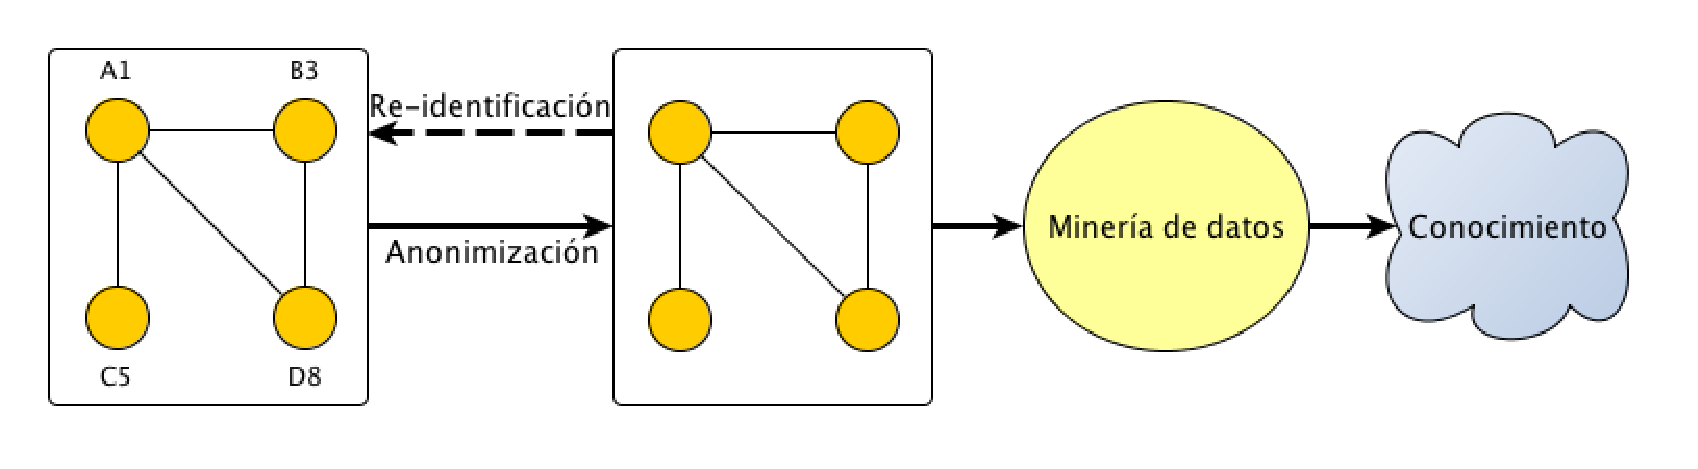
\includegraphics[width=0.8\textwidth]{figs/intro-1}
	\caption{Pie de la imagen.}
	\label{fig:context-anoni1}
\end{figure}

\subsection{Ejemplo de subsection}

Aunque se han realizado importantes avances en preservaci�n de la privacidad en publicaci�n de datos, tales como el modelo \textit{k}-anonymity \cite{Sweeney:2002}.

Un ejemplo de pseudo-c�digo se puede encontrar en el C�digo \ref{code:RandomSwitch-1}

\begin{algorithm}
	\caption{Pseudoc�digo del algoritmo \textit{Random Switch}}
	\label{code:RandomSwitch-1}
	\begin{algorithmic}
		\REQUIRE{El grafo original $G$ y el porcentaje de anonimizaci�n $p$ que se desea aplicar.}
		\ENSURE{El grafo $G$ anonimizado.}
		\STATE $num = round(G.num\_edges() * p)$
		\STATE $i = 0$
		\WHILE {$i < num$}
		\STATE {$e_{1} = G.random\_edge()$}
		\STATE $e_{2} = G.random\_edge()$
		\STATE $new\_e_{1} = (e_{1}.origen, e_{2}.origen)$
		\STATE $new\_e_{2} = (e_{1}.destino, e_{2}.destino)$
		\IF {$!G.exist(new\_e_{1})$ \AND $!G.exist(new\_e_{2})$}
		\STATE $G.add\_edge(new\_e_{1})$
		\STATE $G.add\_edge(new\_e_{2})$
		\STATE $G.delete\_edge(e_{1})$
		\STATE $G.delete\_edge(e_{2})$
		\STATE $i=i+1$
		\ENDIF
		\ENDWHILE
		\RETURN $G$
	\end{algorithmic}
\end{algorithm}

Un ejemplo de tabla se puede ver en la Tabla \ref{table:ejemplo_vertex_refi_query}

\begin{table}
	\centering{}
	\begin{tabular}{ l || c | c | l }
		\hline
		Node ID & $\mathcal{H}_{0}$ & $\mathcal{H}_{1}$ & $\mathcal{H}_{2}$ \\
		\hline
		\hline
		Alice & $\epsilon$ & 1 & \{4\}  \\
		\hline
		Bob & $\epsilon$ & 4 & \{1, 1, 4, 4\}  \\
		\hline
		Carol & $\epsilon$ & 1 & \{4\}  \\
		\hline
		Dave & $\epsilon$ & 4 & \{2, 4, 4, 4\}  \\
		\hline
		Ed & $\epsilon$ & 4 & \{2, 4, 4, 4\}  \\
		\hline
		Fred & $\epsilon$ & 2 & \{4, 4\}  \\
		\hline
		Greg & $\epsilon$ & 4 & \{2, 2, 4, 4\}  \\
		\hline
		Harry & $\epsilon$ & 2 & \{4, 4\}  \\
		\hline
	\end{tabular}
	\caption{\textit{Vertex refinement queries}.}
	\label{table:ejemplo_vertex_refi_query}
\end{table}

% bibliografia
\addcontentsline{toc}{chapter}{Bibliografía}
\bibliographystyle{plain}
\bibliography{referencias}

\end{document}